\documentclass[11pt,a5paper,landscape]{article}

\usepackage{main}
\usepackage{exercices}

% --------------------------------------------------
% Informations du document
% --------------------------------------------------
\renewcommand{\typedocument}{Exercices}
\renewcommand{\classe}{6e}
\renewcommand{\titre}{Exercices - Energie}

\begin{document}

\setlist[enumerate]{topsep=0pt,itemsep=10pt,parsep=0pt,partopsep=0pt,leftmargin=*}

\setlength{\columnsep}{1cm}

\begin{multicols*}{2}

% ----- Exercice 1 -----

\exercice{Formes et sources d'énergie}

\question{Quelles sont les 6 formes d'énergie ?}

\question{Classer les sources d’énergie suivantes dans un tableau à deux colonnes selon qu’elles soient renouvelables ou non renouvelables:}
\textit{Soleil, uranium, eau, pétrole, charbon, gaz, vent.}

% ----- Exercice 2 -----

\exercice{Dynamo}

Morgane a acheté une lampe dynamo pour son vélo. Lorsqu'elle pédale, la dynamo convertit le mouvement en électricité qui alimente la lampe pour éclairer la route. A chaque étape, de l'énergie thermique est perdue.

\question{Quelle énergie est liée au mouvement des roues du vélo ?}

\question{Remplir le schéma suivant en indiquant les différentes formes d'énergie.}

\vspace*{-2.5em}

\begin{center}
    
\includegraphics[width=10cm]{images/3.png}
\end{center}

% ----- Exercice 3 -----

\exercice{Marathon}

Sébastien court un marathon. Pour se préparer, il mange une barre de céréales avant la course.

\question{Quelle forme d'énergie est contenue dans la barre de céréales ?}

\question{Remplir le schéma suivant en indiquant les différentes formes d'énergie.}

\vspace{-1.5em}

\begin{center}
    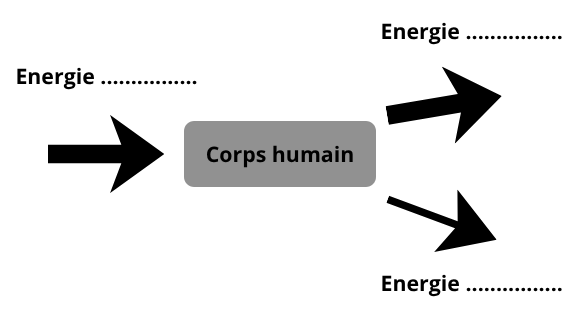
\includegraphics[width=6cm]{images/2.png}
\end{center}

\vspace*{-2em}

% ----- Exercice 4 -----

\exercice{Conservation d'énergie}

\question{En quelle forme d'énergie une lampe transforme-t-elle l'énergie électrique ?}

\question{En quelle forme d'énergie un panneau photovoltaïque transforme-t-il l'énergie lumineuse ?}

\question{Si on éclaire un panneau photovoltaïque avec une lampe, et que cette lampe est branchée au panneau, est-ce qu’on pourrait avoir de l’énergie à l’infini ? Pourquoi ?}


\end{multicols*}
\end{document}